\chapter{Go Programlama Dili}
% ///////////////////////////////////////////////////////////////////////////
% GOLANG
% INDIRME VE KURULUM
% ///////////////////////////////////////////////////////////////////////////

\begin{figure}[!htb]
    \centering
    
\includegraphics[width=1\linewidth]{00-images/00-golang.png}
    \caption{Golang}
    \label{fig:my_label}
\end{figure}

% ///////////////////////////////////////////////////////////////////////////
% ILK PROGRAM
% ///////////////////////////////////////////////////////////////////////////

\section{Golang Kod Örneği}

\lstinputlisting[language=Go]{codes/00-hello_world.go}
\captionof{table}{Merhaba Dünya}

Package main Go programımızın başlangıç noktasıdır ve yazdığımız programın bir executable program olduğunu belirtir ve main fonksiyonunu çalıştırır.
Yazdığımız kodu bir kütüphane olarak paylaşacağımızda ise bir main fonksiyon atamamıza gerek yoktur ve bu yüzden package main olarak tanımlamamızada gerek yoktur. 
import kelimesi dışarıdan kullanıcağımız programa bir paket eklemek istediğimizde kullanılır.
"fmt" kelimesi ise "Format" paketinin kısaltmasıdır. "Format" paketi genel olarak input ve output değerlerinin düzenlenerek yazdırılmasını sağlayan pakettir. 
Main fonksiyonu programımızın ilk olarak çalıştırılan başlangıç noktasıdır ve herhangi bir şekilde değer atanmaz ve aynı şekilde değer de döndürmez 
fmt paketinin içinde yer alan "Print Line" ın kısaltılmışı olan Println  fonksiyonu çağrılarak verilen string değerinin yazdırılmasını sağlar.
go run komutu $"hello\_world.go"$ dosyasının derlenmesi ve sonucun yazdırılmasını sağlar.

\vspace{10mm}
% ///////////////////////////////////////////////////////////////////////////
% INDIRME VE KURULUM
% ///////////////////////////////////////////////////////////////////////////
\section{Indirme ve Kurulum}

% Download 1
\begin{figure}[!htb]
    \centering
    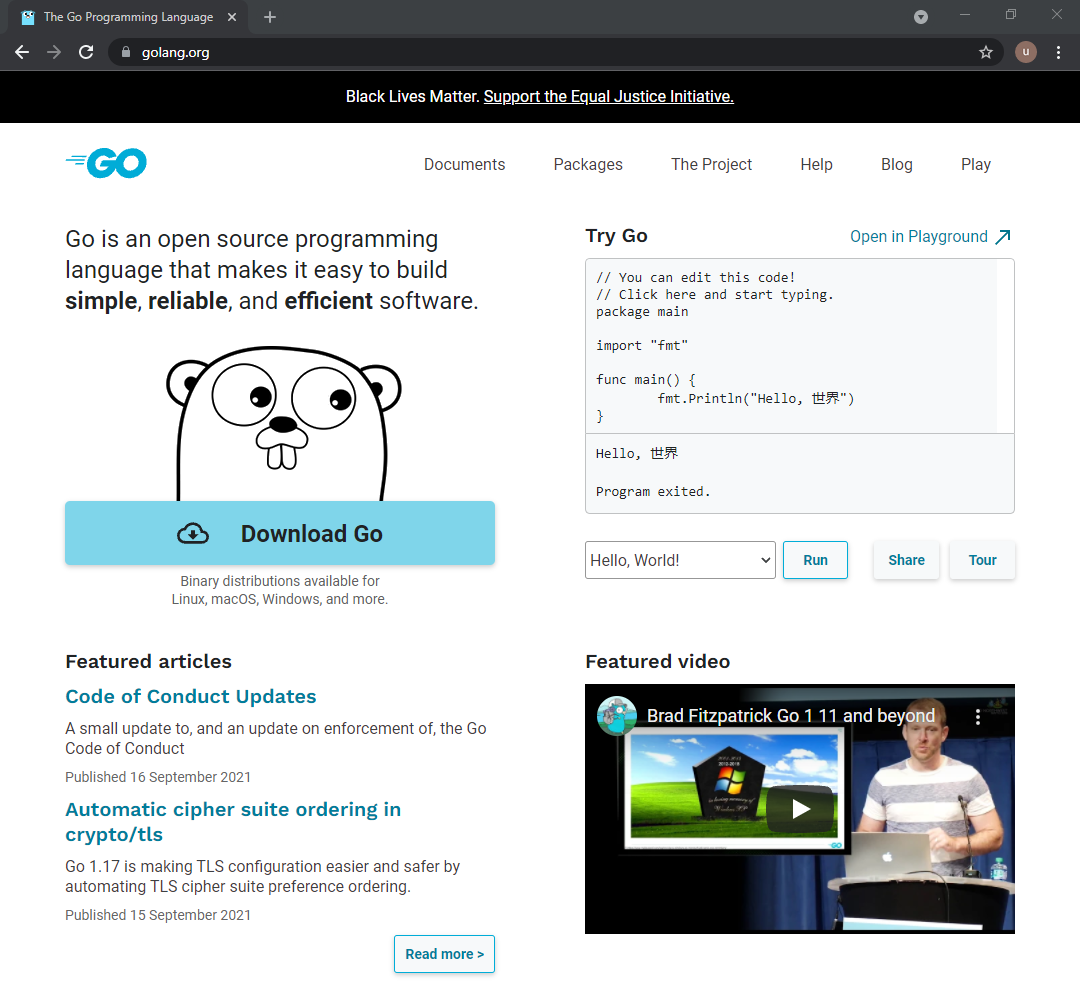
\includegraphics[width=1\linewidth]{00-images/01-download.png}
    \caption{Go programlama dilinin Compiler ını indirebilmek için golang.org sitesinin "Download Go" linkini tıklıyoruz. }
    \label{fig:my_label}
\end{figure}

\vspace{10mm}

\begin{figure}[!htb]
    \centering
    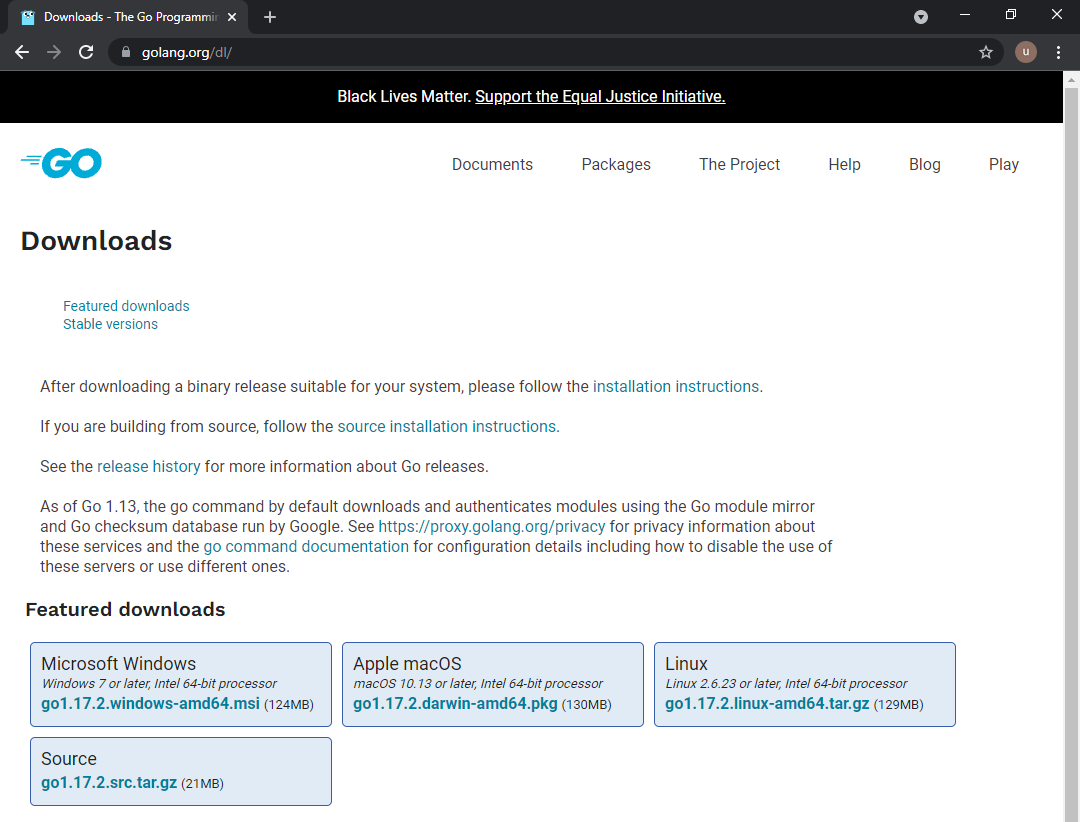
\includegraphics[width=1\linewidth]{00-images/02-download.png}
    \caption{İşletim sistemimize (Windows, macOS, Linux) göre kurulum dosyasını indiriyoruz. }
    \label{fig:my_label}
\end{figure}

\vspace{10mm}

% Installation 1
\begin{figure}[!htb]
    \centering
    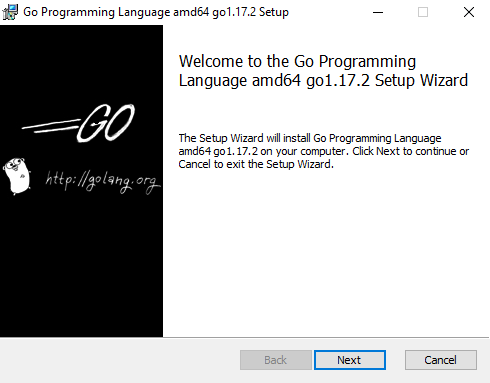
\includegraphics[width=0.6\linewidth]{00-images/03-installation.png}
    \caption{Kurulum dosyasının Next butonuna tıklıyoruz. }
    \label{fig:my_label}
\end{figure}

\vspace{5mm}

% Installation 2
\vspace{10mm}

\begin{figure}[!htb]
    \centering
    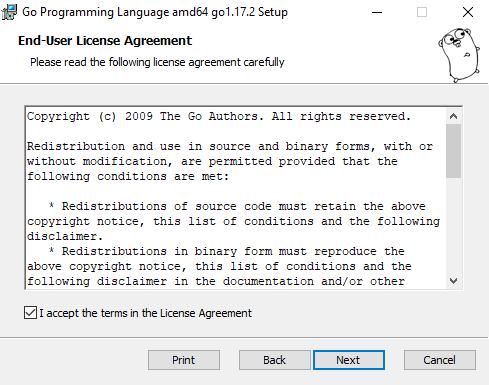
\includegraphics[width=0.6\linewidth]{00-images/04-installation.png}
    \caption{Lisans anlaşmasını kabul edip, Next butonuna tıklıyoruz. }
    \label{fig:my_label}
\end{figure}

\vspace{5mm}

% Installation 3

\begin{figure}[!htb]
    \centering
    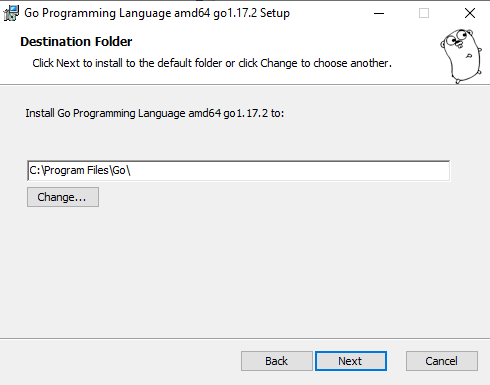
\includegraphics[width=0.6\linewidth]{00-images/05-installation.png}
    \caption{Derleyicinin bilgisayarda hangi alana kurulucağını seçip, Next butonuna tıklıyoruz.}
    \label{fig:my_label}
\end{figure}

\vspace{5mm}

% Installation 4
\vspace{10mm}

\begin{figure}[!htb]
    \centering
    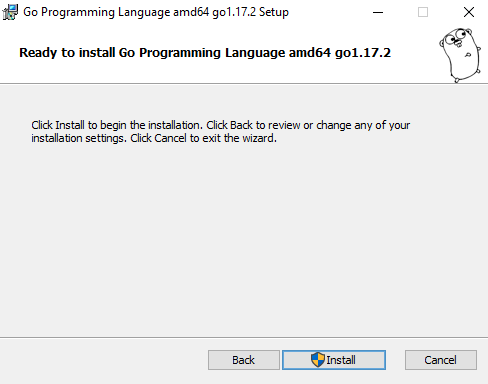
\includegraphics[width=0.6\linewidth]{00-images/06-installation.png}
    \caption{Kurulum için Install butonuna tıklıyoruz.}
    \label{fig:my_label}
\end{figure}

\vspace{5mm}

% Installation 5
\vspace{10mm}

\begin{figure}[!htb]
    \centering
    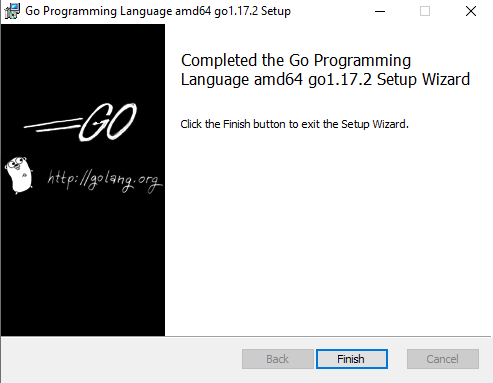
\includegraphics[width=0.6\linewidth]{00-images/07-installation.png}
    \caption{Son olarak Finish butonuna tıklıyoruz ve artık Go Dilinin derleyicisi kurulmuş oldu.}
    \label{fig:my_label}
\end{figure}

\vspace{5mm}

% ///////////////////////////////////////////////////////////////////////////
% VERI TIPLERI
% ///////////////////////////////////////////////////////////////////////////

\vspace{15mm}
\section{Veri Tipleri}
\vspace{7mm}

\begin{table}[!htb]
\begin{tabular}{|lcccc|}
\hline
\multicolumn{5}{|c|}{\textbf{Unsigned Integer}}                                                                                                                                                                 \\ \hline
\multicolumn{1}{|l|}{}                          & \multicolumn{1}{c|}{\textbf{uint8}} & \multicolumn{1}{c|}{\textbf{uint16}} & \multicolumn{1}{c|}{\textbf{uint32}} & \textbf{uint64}                           \\ \hline
\multicolumn{1}{|l|}{\textbf{Başlangıç Değeri}} & \multicolumn{1}{l|}{0}              & \multicolumn{1}{l|}{0}               & \multicolumn{1}{l|}{0}               & \multicolumn{1}{l|}{0}                    \\ \hline
\multicolumn{1}{|l|}{\textbf{Bitiş Değeri}}     & \multicolumn{1}{l|}{255}            & \multicolumn{1}{l|}{65535}           & \multicolumn{1}{l|}{4294967295}      & \multicolumn{1}{l|}{18446744073709551615} \\ \hline
\multicolumn{5}{|c|}{\textbf{Integer}}                                                                                                                                                                          \\ \hline
\multicolumn{1}{|l|}{}                          & \multicolumn{1}{c|}{\textbf{int8}}  & \multicolumn{1}{c|}{\textbf{int16}}  & \multicolumn{1}{c|}{\textbf{int32}}  & \textbf{int64}                            \\ \hline
\multicolumn{1}{|l|}{\textbf{Başlangıç Değeri}} & \multicolumn{1}{c|}{-128}           & \multicolumn{1}{c|}{-32768}          & \multicolumn{1}{c|}{-2147483648}     & -9223372036854775808                                         \\ \hline
\multicolumn{1}{|l|}{\textbf{Bitiş Değeri}}     & \multicolumn{1}{c|}{127}            & \multicolumn{1}{c|}{32767}           & \multicolumn{1}{c|}{2147483647}      & 9223372036854775807                                         \\ \hline
\multicolumn{5}{|c|}{\textbf{Float}}                                                                                                                                                                            \\ \hline
\multicolumn{1}{|l|}{}                          & \multicolumn{2}{c|}{\textbf{float32}}                                      & \multicolumn{2}{c|}{\textbf{float64}}                                            \\ \hline
\multicolumn{1}{|l|}{\textbf{Başlangıç Değeri}} & \multicolumn{2}{c|}{-3.4E+38}                                              & \multicolumn{2}{c|}{-1.7E+308}                                                   \\ \hline
\multicolumn{1}{|l|}{\textbf{Bitiş Değeri}}     & \multicolumn{2}{c|}{3.4E+38}                                               & \multicolumn{2}{c|}{1.7E+308}                                                    \\ \hline
\end{tabular}
\end{table}


\vspace{20mm}
\textbf{String Veri Tipi}
\vspace{7mm}

Go dilinde String Veri Tipi karakterleri kelimeleri veya cümleleri tanımlamak için kullanılır ve bunlar tanımlanırken ilk program da verdiğimiz örnekteki gibi "Hello World" çift tırnak içinde tanımlanırlar.

\vspace{5mm}
Go dilinde String Veri Tipi UTF-8 olarak kodlu bir biçimdedir. UTF-8 8 bitlik bir alana sahiptir.


\vspace{20mm}
\textbf{Boolean Veri Tipi}
\vspace{7mm}

Go dilinde Veri Tiplerinin karşılaştırılmasını sağlayan ve bunun sonucunuda "true" doğru ve "false" yanlış olarak geri döndüren veri tipine Boolean Veri Tipi diyoruz.

\vspace{10mm}
Go dilinde İki veri tipini karşılaştırmada $"==", "!=", "<", "<=", ">="$ işaretlerini kullanıyoruz

\vspace{10mm}
Go dilinde $"=="$ işareti iki veri tipinin aynı veri tiplerine sahip olup olmadığını vede aynı değerleri tutup tutmadığını değer olarak "true" yada "false" geri döndürür.

\vspace{10mm}
Go dilinde $"!="$ işareti iki veri tipinin farklı veri tiplerine sahip olup olmadığını vede farklı değerleri tutup tutmadığını değer olarak "true" yada "false" geri döndürür.

\vspace{10mm}
Go dilinde $"<", ">"$ işaretleri bir verinin diğer veri den daha büyük veya daha küçük olup olmadığını ölçer ve bunun sonucunda değer olarak "true" yada "false" geri döndürür.

\vspace{10mm}
Go dilinde $"<=", ">="$  işaretleri bir verinin diğer veri den büyük eşit yada küçük eşit olup olmadığını ölçer ve bunun sonucunda değer olarak "true" yada "false" geri döndürür.
\vspace{10mm}

\lstinputlisting[language=Go]{codes/01-data_types.go}
\captionof{table}{Veri Tipleri}


% ///////////////////////////////////////////////////////////////////////////
% DEGISKEN ATAMA
% ///////////////////////////////////////////////////////////////////////////

\section{Değişken Atama}

\vspace{10mm}

Go dilinde değişken atamaları derleme zamanında statik olarak yapılır. Değişken atama çeşitleri var ve const olarak ikiye ayrılır. 

\vspace{20mm}


\textbf{Variables "var"}
\vspace{10mm}

var ile değişken ataması yaptığımızda atanan değer veri tipi aynı kalmak şartıyla değiştirilebilir.
\vspace{10mm}

\lstinputlisting[language=Go]{codes/02-var_assignment.go}
\captionof{table}{Var Değişken Değer Ataması}


\vspace{20mm}
\textbf{Constants "const"}
\vspace{10mm}

const ile değişken ataması yaptığımızda atanan değer sabit bir şekilde kalır ve değiştirilemez.  
\vspace{5mm}
\lstinputlisting[language=Go]{codes/02-const_assignment.go}
\captionof{table}{Const Sabit Değer Ataması}
\vspace{10mm}

\vspace{10mm}
\textbf{Kısaltılmış Değer Ataması}
\vspace{7mm}

Go dilinde ":=" işareti kullanılarak daha kısa bir şekilde değer ataması mümkündür. 
\vspace{5mm}

\lstinputlisting[language=Go]{codes/02-shorter_assignment.go}
\captionof{table}{Kısaltılmış Değer Ataması}


\vspace{8mm}
\textbf{Çoklu "var" Değer Ataması}
\vspace{7mm}

Go dilinde birden fazla değerin var kullanılarak tek seferde atanması mümkündür.
\vspace{5mm}

\lstinputlisting[language=Go]{codes/02-multiple_variable_assingment.go}
\captionof{table}{Birden Fazla Değişken Değer Ataması}

\vspace{10mm}
\textbf{Çoklu "const" Değer Ataması}
\vspace{7mm}

Go dilinde birden fazla değerin const kullanılarak tek seferde atanması mümkündür.
\vspace{5mm}
\lstinputlisting[language=Go]{codes/02-multiple_constant_assingment.go}
\captionof{table}{Birden Fazla Sabit Değer Ataması}


\vspace{20mm}
\textbf{Global Scope Değer Ataması}
\vspace{7mm}

Go dilinde fonksiyon dışlarında global değer atamaları yapılabilir ve bu atanan değerlere fonksiyonlardan erişim sağlanabilir.
\vspace{10mm}
\lstinputlisting[language=Go]{codes/02-global_scope.go}
\captionof{table}{Global Scope Değer Ataması}


\vspace{10mm}
\textbf{Local Scope Değer Ataması}
\vspace{5mm}

Go dilinde fonksiyon içlerinde local değer atamaları yapılabilir ve bu atanan değerlere direkt olarak ancak fonksiyon içerisinden erişim sağlanabilir.
\vspace{5mm}

\lstinputlisting[language=Go]{codes/02-local_scope.go}
\captionof{table}{Local Scope Değer Ataması}

% ///////////////////////////////////////////////////////////////////////////
% KONTROL YAPILARI
% ///////////////////////////////////////////////////////////////////////////

\section{Kontrol Yapilari}
\vspace{5mm}

Go dilinde complex problemlerle karşılaşabiliriz bunların çözümünde "for, if, switch" gibi kontrol yapılarını kullanabiliriz. 

\vspace{20mm}


\textbf{Döngüler "for"}
\vspace{7mm}

for ile değişkenlerimizi döngüde tutarak istediğimiz işlemleri birden fazla işlem basamağıyla gerçekleştirebiliriz.
\vspace{5mm}
\lstinputlisting[language=Go]{codes/05-for_loop.go}
\captionof{table}{For Döngüsü}


\vspace{10mm}
\textbf{Döngüler "while"}
\vspace{5mm}

Go dilinde diğer dillerde olduğu gibi ayrı bir "while" döngü yapısı kullanılmak yerine for döngüsü ile while döngüsünü oluşturabiliyoruz.
\vspace{5mm}
\lstinputlisting[language=Go]{codes/05-while_loop.go}
\captionof{table}{While Döngüsü}


\vspace{10mm}
\textbf{Karar Yapısı "if,else if, else"}
\vspace{5mm}

if, else if, else ile değişkenlerimizin doğruluk sağlayıp sağlamamasına göre işlem karar mekanizmaları oluşturabiliriz.
\vspace{5mm}

\lstinputlisting[language=Go]{codes/05-if_else.go}
\captionof{table}{If, Else Yapıları}

\vspace{10mm}
\textbf{Karar Yapısı "switch case"}
\vspace{5mm}

switch case ile değişkenlerimizin doğruluk sağlayıp sağlamamasına göre işlem karar mekanizmaları oluşturabiliriz.
\vspace{5mm}
\lstinputlisting[language=Go]{codes/05-switch_case.go}
\captionof{table}{Switch Case Yapısı}

% ///////////////////////////////////////////////////////////////////////////
% ARRAYS, SLICES, MAPS
% ///////////////////////////////////////////////////////////////////////////

\section{Arrays, Slices, Maps}
\vspace{5mm}

Go dilinde verileri gruplandırmak ve bir arada tutmak için "arrays, slices, maps" gibi veri yapılarını kullanıyoruz. 
\vspace{10mm}

\textbf{Diziler "arrays"}
\vspace{5mm}

Go dilinde sabit uzunluklu diziler tanımlayabiliriz.
\vspace{5mm}

\lstinputlisting[language=Go]{codes/06-fixed_size_array.go}
\captionof{table}{Sabit Uzunlukdaki Diziler}


\vspace{10mm}
\textbf{Slices}
\vspace{5mm}

Go dilinde dizilerin uzerine inşa edilmiş slice yapısı bulunmaktadır. Bu yapılar dinamik olarak uzunluğunu arttırabilir yada azaltabilir.
\vspace{5mm}

\lstinputlisting[language=Go]{codes/06-slices.go}
\captionof{table}{Slices}

\vspace{20mm}
\textbf{Ekleme "append"} append ile dizilerimize veri ekleyebiliyoruz.
\vspace{5mm}
\lstinputlisting[language=Go]{codes/06-append.go}
\captionof{table}{Diziye Veri Ekleme}


\vspace{10mm}
\textbf{Çok Boyutlu Diziler}
\vspace{5mm}

Multi Dimensional Arrays ile çok boyutlu veri dizileri oluşturabiliyoruz.
\vspace{5mm}
\lstinputlisting[language=Go]{codes/06-multi_dimensional.go}
\captionof{table}{Çok Boyutlu Diziler}


\vspace{20mm}
\textbf{Maps}
\vspace{5mm}

Maps ile anahtar değer ilişkisiyle veri tutabilen veri yapısıdır. Bilgisayar bilimlerinde genel olarak Hash Table olarak bilinir
\vspace{5mm}
\lstinputlisting[language=Go]{codes/06-map.go}
\captionof{table}{Map}


\vspace{10mm}
\textbf{Append, Delete}
\vspace{5mm}

Maps de veri eklemeyi yeni bir anahtar değer ekliyerek vede silmek için ise Delete fonksiyonunu kullanıyoruz.
\vspace{5mm}
\lstinputlisting[language=Go]{codes/06-map_append_delete.go}
\captionof{table}{Map Ekleme ve Silme}

% ///////////////////////////////////////////////////////////////////////////
% FONKSIYONLAR
\newpage
% ///////////////////////////////////////////////////////////////////////////

\section{Fonksiyonlar}

\vspace{10mm}

Go dilinde "functions" olarak adlandırılan kod blokları bulunmaktadır. Fonksiyonlar genel olarak karmaşık problemlerin çözümünde modülerlik açısından karmaşıklığın azaltılması ve kodun tekrar kullanılabilirliğinin arttırılması için kullanılır.
\vspace{5mm}

Bu kod blokları birden fazla parametre alabiliceği gibi hiç parametre almayadabilir. Aynı şekilde birden fazla değer geri döndürebiliceği gibi hiç geri değer döndürmeyedebilir.

\vspace{20mm}


\textbf{Fonksiyonlar}
\vspace{5mm}

Go dilinde şu ana kadar sadece Main Fonksiyonunu kullanıyorduk. 
\vspace{5mm}
\lstinputlisting[language=Go]{codes/07-main_function.go}
\captionof{table}{Main Function}

\vspace{10mm}
\textbf{Değer Almayan ve Döndürmeyen Fonksiyonlar}
\vspace{5mm}

Go dilinde fonksiyonların herhangi bir değer alması veya döndürmesi zorunlu değildir.
\vspace{5mm}
\lstinputlisting[language=Go]{codes/07-dummy_func.go}
\captionof{table}{Dummy Function}


\vspace{10mm}
\textbf{Değer Alan Fonksiyonlar}
\vspace{5mm}

Go dilinde bir veya birden fazla değer alan fonksiyonlar yazılabilir.
\vspace{5mm}
\lstinputlisting[language=Go]{codes/07-func_args.go}
\captionof{table}{Fonksiyon Argumanları}


\vspace{10mm}
\textbf{Değer Döndüren Fonksiyonlar}
\vspace{5mm}

Değer döndüren fonksiyonlarda fonksiyon ismi tanımlandıktan sonra döndürülücek değer tipleri tanımlaması yapılır.
\vspace{5mm}
\lstinputlisting[language=Go]{codes/07-return_value.go}
\captionof{table}{Değer Döndüren Fonksiyonlar}

\vspace{20mm}
\textbf{Birden Fazla Değer Alan ve Birden Fazla Değer Döndüren Fonksiyonlar}
\vspace{5mm}

Go dilinde fonksiyonlar birden fazla değer alabildiği gibi birden fazla değer döndürebilirler.
\vspace{5mm}


\lstinputlisting[language=Go]{codes/07-multiple_args_returns.go}
\captionof{table}{Birden Fazla Değer Alan ve Birden Fazla Değer Döndüren Fonksiyonlar}


\vspace{10mm}
\textbf{Defer, Panic ve Recover}
\vspace{5mm}

\textbf{Defer} kullandığımız fonksiyon çağırıldığı fonksiyon bloğunun bitmesini bekler ve ardından çalışır.
\vspace{5mm}
\lstinputlisting[language=Go]{codes/07-defer.go}
\captionof{table}{Defer}

\vspace{10mm}
\textbf{Panic} çalışma zamanı hatasına sebep olur.
\vspace{5mm}
\lstinputlisting[language=Go]{codes/07-panic.go}
\captionof{table}{Panic}

\vspace{10mm}
\textbf{Recover} panic kullanarak sebep olduğumuz çalışma zamanı hatasından defer ve recover fonksiyonlarıni kullanarak kurtuluruz.
\vspace{5mm}
\lstinputlisting[language=Go]{codes/07-recover.go}
\captionof{table}{Recover}

% ///////////////////////////////////////////////////////////////////////////
% POINTERS
% ///////////////////////////////////////////////////////////////////////////
\section{Pointers}
\vspace{5mm}

Go dilinde "pointer" referansları bulunmaktadır ve bu referanslar kullandığımız değerin bellekteki adresini temsil eder.
\vspace{20mm}

\textbf{\& Referans Operatörü } 
\vspace{7mm}

\& operatörü oluşturduğumuz değerlerin bellek adreslerine ulaşmamızı sağlar.

\vspace{5mm}
\lstinputlisting[language=Go]{codes/08-and_operator.go}
\captionof{table}{\& Operatörü}

\vspace{10mm}

\textbf{* Referans Operatörü } 
\vspace{7mm}

* operatörü adres referans bilgisine sahip olduğumuz değerleri bize verir.

\vspace{5mm}
\lstinputlisting[language=Go]{codes/08-multiply_operator.go}
\captionof{table}{\* Operatörü}


\vspace{10mm}
\textbf{Referans Örneği}
\vspace{5mm}

Aşağıdaki örnekde adres değeri kullanılarak değişken değeri değiştirilmiştir.

\vspace{5mm}
\lstinputlisting[language=Go]{codes/08-pointer_example.go}
\captionof{table}{Pointer Örneği}

\vspace{10mm}

% ///////////////////////////////////////////////////////////////////////////
% STRUCT VE INTERFACE
\newpage
% ///////////////////////////////////////////////////////////////////////////

\section{Struct ve Interface}
\vspace{5mm}

Struct Go Dilinde Verilerin Düzenli Bir Şekilde Tutulması İçin Kullanılır.
\vspace{7mm}


\vspace{5mm}
\lstinputlisting[language=Go]{codes/09-struct.go}
\captionof{table}{Struct}

\vspace{10mm}

\textbf{Struct Örneği}
\vspace{10mm}

Aşağıdaki örnekde struct direk olarak değişken tipleri belirtilmiş ve bir değişkene atanmıştır.

\vspace{10mm}
\lstinputlisting[language=Go]{codes/09-struct_example.go}
\captionof{table}{Struct Örneği}

\vspace{10mm}

Interface Go Dilinde bir veya daha fazla Methodun Method İmzaları kullanılarak bir arada toplanması için kullanılan bir yapıdır.
\vspace{10mm}

\lstinputlisting[language=Go]{codes/09-interface.go}
\captionof{table}{Interface}

\vspace{10mm}

\textbf{Interface Örneği} 
\vspace{5mm}

Aşağıdaki interface örneğinde kare ve dairenin alanı struct olarak tanımlandı ve method imzaları olan 'square' and 'circle' method koleksiyonu olan 'shape' üzerinde tanımlaması yapıldı.

\lstinputlisting[language=Go]{codes/09-interface_example.go}
\captionof{table}{Interface Örneği}

\vspace{10mm}

% ///////////////////////////////////////////////////////////////////////////
% CONCURRENCY
% ///////////////////////////////////////////////////////////////////////////

\section{Concurrency}
\vspace{5mm}

Goroutines Go dilinde threadlerin yerine kullanabiliceğimiz daha az kaynak tüketimi olan goroutine(sanal thread) ler bulunmaktadır. Her bir programın içerisinde en az bir goroutine bulunmaktadır ve bu goroutine 'main goroutine' olarak adlandırılır.Diğer bütün goroutineler 'main goroutine' in altında çalışırlar.

\vspace{5mm}
\lstinputlisting[language=Go]{codes/10-goroutines.go}
\captionof{table}{Goroutines}

\vspace{10mm}

\textbf{Goroutines Örnek}
\vspace{10mm}

Aşağıdaki örnekde multithreading i simüle edebilmek için 'time.Sleep' fonksiyonundan yararlanılmıştır fakat bu fonksiyonun kaynak tüketimi yüksektir bu yüzden kaynak tüketimi daha az olan  'sync.WaitGroup' fonksiyonlarını kullanacağız.

\vspace{10mm}

\lstinputlisting[language=Go]{codes/10-goroutines_example_1.go}
\captionof{table}{Goroutine Örneği}

\vspace{10mm}

\textbf{Goroutines Örnek 2}
\vspace{10mm}

Aşağıdaki örnekde 'time.Sleep' fonksiyonu yerine  'sync.WaitGroup' fonksiyonları kullanıldı.

\vspace{10mm}
\lstinputlisting[language=Go]{codes/10-goroutines_example_2.go}
\captionof{table}{Goroutine Örneği 2}
\vspace{10mm}

\textbf{Channels}
\vspace{5mm}

Channels, eşzamanlı goroutinleri birbirine bağlayan kanallardır. Bir goroutinden Channels üzerinden değerler gönderebilir ve bu değerleri başka bir goroutine ile Channels üzerinden alabilirsiniz.
\vspace{10mm}

\lstinputlisting[language=Go]{codes/10-channels.go}
\captionof{table}{Channels}

\vspace{10mm}

\textbf{Channels Örnek}

\vspace{10mm}
\lstinputlisting[language=Go]{codes/10-channels_example.go}
\caption{Channels Örneği}

\vspace{10mm}

% ///////////////////////////////////////////////////////////////////////////
